\documentclass[10pt]{article}
\usepackage{tmlr}
% \usepackage[preprint]{tmlr}

\usepackage{hyperref}
\usepackage{url}
\usepackage{amsmath,amssymb,mathtools}
\usepackage{booktabs}
\usepackage{array}
\usepackage{graphicx}
\usepackage{amsthm}
\newtheorem{proposition}{Proposition}

\newcommand{\R}{\mathbb{R}}
\newcommand{\jvp}{\textsc{jvp}}
\newcommand{\fd}{\textsc{fd}}
\newcommand{\eps}{\varepsilon}

\title{A Step-Selection Trilemma for Finite-Difference Generator Curvature}

\author{\name Anonymous}

\def\month{06}
\def\year{2026}
\def\openreview{}

\begin{document}
\maketitle

\begin{abstract}
Second-order generator geometry is in live use: geodesic interpolation, curvilinear
edits, and Hessian disentanglement priors all reach for the curvature of the generated
manifold, and the estimator a practitioner reaches for is a central finite difference. We
show that on real generators this estimator faces a step-selection \emph{trilemma}: the steps
that best preserve curvature magnitude, signed bias, and the ranking of directions are
systematically different, so no single step gets all three right at once. The three criteria are
optimized at three different steps (magnitude-best $\delta=3.0$, bias-best $\delta=2.0$,
rank-best $\delta\approx0.2$). The magnitude error has a $\sqrt{\eps_{\mathrm{mach}}}$ floor
(classical; Proposition~\ref{prop:floor} proves it exists), measured at $\geq45\%$ on StyleGAN
($47\%$ on a matched fp32/fp64 control, so precision does not remove it); the signed bias crosses
zero between the magnitude- and rank-best steps; and a fixed-step finite difference recovers the
ranking well (Spearman up to $0.98$).
The conflict reproduces across three StyleGAN-bedroom seeds, three full-resolution FFHQ seeds,
and lower-detail controls, at generator-dependent step values. As an exact reference we use
composed forward-mode automatic differentiation -- standard nested-\jvp{} machinery
\citep{pearlmutter1994,fike2011,baydin2018,cobb2024}, applied to generator curvature by
\citet{lee2023} -- step-free and exact to machine precision (validated to $2.5\times10^{-17}$
against an analytic ground truth, vs the best finite difference's $8.6\times10^{-9}$). Using this reference we run a replication audit of whether curvature predicts edit nonlinearity
beyond first-order displacement; the signal is significant on two of five anchors but does not
transfer (cross-anchor $95\%$ CI $[-0.09,+0.43]$ spans zero), and a fixed-step finite difference
returns the same non-transferring answer. The instrument's value is on the magnitude and sign
axes, where no step is correct, rather than on this rank-level question. We
recommend that second-order generator-geometry reports use an exact or step-validated
estimator for magnitude and sign, report the step axis, and replicate direction-level claims
across anchors.
\end{abstract}

\section{Introduction}
\label{sec:intro}
Editing methods for pretrained GANs increasingly treat the latent space as a Riemannian
manifold and reach for its second-order structure. Geodesic interpolation replaces linear
interpolation using a pullback metric \citep{arvanitidis2018,shao2018,chen2018}; curvilinear
edit paths are constructed to be nonlinear by design \citep{aoshima2023}; and second-order
Hessian information is used as a disentanglement prior \citep{peebles2020}. Each of these
needs the curvature of the generator -- the change of the Jacobian along an edit -- and the
estimator a practitioner reaches for is a finite-difference second difference of the
generator.

That estimator has no defensible setting. A curvature estimate must get three things right -- its
magnitude, its sign, and the ranking of directions it induces -- and for the second-order difference on
StyleGAN these three are optimized at \emph{different} steps: no single step preserves all three at once, and
the signed error even changes sign across the usable range (Section~\ref{sec:real},
Table~\ref{tab:trilemma}). The first-order difference of the same code has no such conflict; one step
region is at once accurate, unbiased, and rank-faithful, which is why first-order Jacobians and pullback
metrics have been safe to finite-difference while second-order curvature is not. The magnitude axis of
this conflict is an irreducible relative-error floor of order $\sqrt{\eps_{\mathrm{mach}}}$
(Proposition~\ref{prop:floor}): on StyleGAN no shared step beats a $45\%$ mean error ($38\%$ median),
identical in fp32 and fp64, so the source is the generator's nonlinearity rather than roundoff. Because
no step is defensibly choosable, finite differences cannot yield a curvature one can trust for
magnitude, sign, and ranking at once.
The same qualitative split repeats on two additional StyleGAN-bedroom seeds and on three full-resolution
StyleGAN-FFHQ seeds, with lower-detail FFHQ controls (Appendix~\ref{app:robustness}); the particular best steps change, but the
conflict between magnitude, bias, and ranking does not.

The fix is exact. The second-order term is the directional
derivative of the first, so composing forward-mode automatic differentiation with itself
returns the second-order pushforward to machine precision -- no step, in memory
a small constant multiple of one forward pass (Section~\ref{sec:inst}). We validate it
against a first-order finite-difference control that agrees to $2.4\%$ and against an
analytic referee where it reaches $2.5\times10^{-17}$ while the best finite difference
manages only $8.6\times10^{-9}$.

With the exact second-order quantity in hand, free of the step-selection confound, we
revisit a concrete question a practitioner faces -- does the
curvature of an edit direction predict how \emph{nonlinear} the edit is, how far the
rendered path bows away from the straight chord? -- as an audit of what the instrument
changes.

Our main finding is an empirical step-selection trilemma for finite-difference generator
curvature; we establish it against an exact composed-\jvp{} reference and use that reference
to audit one curvature--nonlinearity claim. Concretely:

\begin{itemize}
\item An empirical step-selection \emph{trilemma} for finite-difference generator curvature
(the paper's main contribution): magnitude, signed bias, and rank fidelity are optimized at
different steps (Table~\ref{tab:trilemma}), while the first difference of the same code is
accurate, unbiased, and rank-faithful together near one step ($2.4\%$). Its magnitude axis is
the classical $\sqrt{\eps_{\mathrm{mach}}}$ second-difference floor \citep{higham2002,press2007},
restated as Proposition~\ref{prop:floor} and measured at $\geq45\%$ on StyleGAN (identical in
fp32/fp64); the bias and rank axes are empirical. The conflict repeats on two more bedroom seeds
and three full-resolution FFHQ seeds with lower-detail controls
(Sections~\ref{sec:fd},~\ref{sec:real}; Appendix~\ref{app:robustness}).
\item An exact reference for that measurement: composed forward-mode AD -- standard
nested-\jvp{} machinery \citep{pearlmutter1994,fike2011,baydin2018,cobb2024}, used by
\citet{lee2023} for generator curvature -- which is step-free and exact to machine precision
at a small constant multiple of one forward pass (Section~\ref{sec:inst}).
\item A deterministic prescription: probing second-order generator geometry calls for the
exact instrument; any method built on a finite-difference generator Hessian -- the Hessian
Penalty \citep{peebles2020} -- inherits the per-sample step-selection ambiguity
(Section~\ref{sec:scope}).
\item A scope delineation (Section~\ref{sec:negative}): the floor is a property of the
estimator, and it bites where curvature \emph{magnitude} or \emph{sign} enters a computation
directly, not where only the cross-direction ranking matters. We make this concrete on one
ML application -- predicting edit nonlinearity from curvature -- where the exact reference and
a fixed-step finite difference return the same (non-transferring) answer, confirming that on a
rank-level task the floor does not change the conclusion.
\end{itemize}

The estimator gap therefore matters for magnitude- and sign-dependent uses of generator
curvature (geodesic energy, curvature-penalty weights); a step-validated finite difference or
the exact reference is needed there, while rank-level uses tolerate finite differences.

\section{Setup}
\label{sec:setup}
Let $G:\R^{d}\to\R^{3HW}$ be a pretrained generator and $z$ a latent code. For a unit
direction $v$ the edit path is $\alpha\mapsto G(z+\alpha v)$. We compare three quantities along
this path at $\alpha=0$.

\paragraph{Prediction target (estimator-free).} The \emph{path nonlinearity} $\mathrm{NL}(z,v)$
is how far the rendered path departs from the straight chord between its endpoints, measured by
rendering only: sample $K$ points $\alpha_k\in[-T,T]$, form the chord between $G(z-Tv)$ and
$G(z+Tv)$, and average the normalized image-space deviation of the interior points from the
chord. This is exactly ``how wrong is linear interpolation'' over the edit range, and it uses
no derivative estimator, so it cannot favor either proxy.

\paragraph{First-order proxy (baseline).} The displacement $\lVert J_z v\rVert =
\lVert\partial_\alpha G\rVert$, the exact first-order \jvp{}. This is the cheap quantity a
practitioner already has.

\paragraph{Second-order proxy.} The curvature magnitude $\lVert\partial_\alpha^2 G\rVert$.
Whether this predicts $\mathrm{NL}$ beyond the first-order proxy is the audit we return
to in Section~\ref{sec:negative}; obtaining it reliably is the problem the instrument solves.

\section{Second differences cannot recover generator curvature}
\label{sec:fd}
The obvious way to obtain $\partial_\alpha^2 G$ without automatic differentiation is a central
second difference, whose accuracy is governed by the classical truncation-versus-cancellation
tradeoff \citep{higham2002,press2007}. It does not work in the precision generators run in.

\begin{proposition}[Second-order non-recoverability]
\label{prop:floor}
Let $f\in C^4$ near $\alpha$ with $f^{(4)}$ bounded and $f''(\alpha)\neq0$, evaluated in
floating point with unit roundoff $\eps_{\mathrm{mach}}$ under a standard rounding model
\citep{higham2002}. The central second difference $D^2_\eps f=\big(f(\alpha+\eps)-2f(\alpha)+
f(\alpha-\eps)\big)/\eps^2$ has relative error
\[
\frac{|D^2_\eps f-f''(\alpha)|}{|f''(\alpha)|}
\;\lesssim\; C_T\,\eps^2 + C_R\,\eps_{\mathrm{mach}}/\eps^2,
\qquad C_T=\frac{|f^{(4)}(\alpha)|}{12\,|f''(\alpha)|},\;\;
C_R=O\!\Big(\frac{|f(\alpha)|}{|f''(\alpha)|}\Big),
\]
whose minimum over the step is of order $\sqrt{C_T C_R\,\eps_{\mathrm{mach}}}$, attained at
$\eps^\star\sim\eps_{\mathrm{mach}}^{1/4}$; no step does better. The central first difference, by
contrast, attains a floor of order $\eps_{\mathrm{mach}}^{2/3}$. For a vector map
$G:\R^{d}\to\R^{3HW}$ the bound holds componentwise, so a single global step is governed by the
worst component.
\end{proposition}

The truncation term $\tfrac{\eps^2}{12}f^{(4)}$ and the cancellation term
$O(\eps_{\mathrm{mach}}|f|/\eps^2)$ cannot be small together; the exponent $\tfrac12$ is intrinsic
to the operation and the constant carries the generator's nonlinearity $|f^{(4)}f|/f''^2$, which is
large for a deep network (derivation in Appendix~\ref{app:deriv}). In double precision the floor is
about $10^{-8}$ in the benign case; in the single precision generators use
($\eps_{\mathrm{mach}}\approx1.2\times10^{-7}$) it is about $3\times10^{-4}$ benign and far worse for
a strongly nonlinear $G$, where Section~\ref{sec:real} measures $\geq45\%$. The first difference is
different: a milder floor $\eps_{\mathrm{mach}}^{2/3}$ with a wide usable window, so first-order
Jacobians are safe to finite-difference while second-order curvature is not. This asymmetry is also
our control: wherever the first-order finite difference agrees with the exact \jvp{}, the pipeline is
correct and any second-order disagreement is real.

To check the constants against ground truth, let $f(\alpha)=[\,e^{0.7\alpha},\sin 3\alpha,
(\alpha+0.4)^3,\tanh 2\alpha,\alpha^2\cos\alpha\,]$, with derivatives known in closed form. At
$\alpha=0.3$ in double precision (Table~\ref{tab:toy}) the central second-order relative error is
U-shaped, bottoming at $8.6\times10^{-9}$ near $\eps=10^{-4}$ and diverging to $0.29$ by
$\eps=10^{-8}$; the composed \jvp{} reaches $2.5\times10^{-17}$, so the best finite difference is
$3.5\times10^{8}$ times worse, matching the Proposition~\ref{prop:floor} bound with the $1/12$
constant.

\begin{table}[h]\centering
\begin{tabular}{rcl}
\toprule
$\eps$ & central \fd{} 2nd-order rel.\ err. & \\
\midrule
$10^{-1}$ & $7.9\times10^{-3}$ & (truncation) \\
$10^{-2}$ & $8.0\times10^{-5}$ & \\
$10^{-4}$ & $8.6\times10^{-9}$ & (best) \\
$10^{-6}$ & $3.0\times10^{-5}$ & \\
$10^{-8}$ & $2.9\times10^{-1}$ & (cancellation) \\
\midrule
composed \jvp & $2.5\times10^{-17}$ & (exact) \\
\bottomrule
\end{tabular}
\caption{Second-order accuracy on the analytic toy at $\alpha=0.3$, double precision. No
finite-difference step approaches the exact composed \jvp{}.}
\label{tab:toy}
\end{table}

\section{The non-recoverability is real on a generator}
\label{sec:real}
On StyleGAN-bedroom at $256{\times}256$ in fp32, the best single step $\delta\!\approx\!3$ shared across
edit directions leaves the central second-difference curvature with a $45\%$ mean relative-error floor
($38\%$ median across directions), rising on both sides and exploding as $\delta\to0$
(Figure~\ref{fig:floor}). On matched inputs the floor is identical in fp32 and fp64 ($47\%$ in both; the
gap from the $45\%$ best-step value reflects the input sample, not precision), confirming it is truncation
against the generator's nonlinearity rather than roundoff. This $\geq45\%$ figure is the \emph{magnitude}
axis of Proposition~\ref{prop:floor}; on a real generator the difficulty is three-fold.

\paragraph{An empirical step-selection trilemma.} Magnitude accuracy is not the only thing a
second-order estimate must get right. A practitioner may need the curvature \emph{magnitude} (geodesic
energy, regularizer strength), its \emph{sign}/unbiasedness (a thresholded decision), or the
\emph{ranking} of directions by curvature (which edit is ``most curved''). Across our $96$
direction--anchor pairs these three criteria are optimized at \emph{different} steps
(Table~\ref{tab:trilemma}): magnitude error is least at $\delta=3.0$ ($45\%$), the signed bias is
smallest at $\delta=2.0$ ($+5\%$), and rank fidelity is highest at $\delta\approx0.2$ (Spearman $0.983$).
The magnitude-optimal step gives lower rank fidelity than the rank-optimal step, while the rank-optimal
step incurs a $355\%$ magnitude error; and the signed bias crosses from underestimation at large steps to
overestimation at small steps, so there is no ``safe side'' to err on. This three-way conflict is
\emph{empirical} -- Proposition~\ref{prop:floor} bounds only the magnitude axis, and the bias and rank
axes are measured rather than proved -- and it is specific to second order: the analogous first-order
quantity is accurate, unbiased, and rank-faithful together in a common region near $\delta=0.02$ ($2.4\%$
error, $-0.0\%$ bias, Spearman $0.999$; right columns of Table~\ref{tab:trilemma}). The first-order
central difference of the same code thus agrees with the exact \jvp{} to $2.4\%$, so the pipeline is
correct and the second-order conflict is genuine. The exact composed-\jvp{} instrument removes the step
axis altogether and serves as the reference against which all three criteria are even defined. These specific
step values are properties of this generator's nonlinearity; what we expect to generalize is the
\emph{existence} of the conflict -- a magnitude floor coexisting with an opposite-signed cancellation
regime -- not the particular steps, which is why we state the trilemma as empirical.

\paragraph{Robustness.} Repeating the same $16$-step sweep on two additional bedroom seeds preserves the
conflict: the magnitude-best step remains $\delta=3.0$ with $51\%$ and $43\%$ mean error, while the
rank-best steps move to $\delta=0.2$ and $\delta=0.3$ and incur $315\%$ and $258\%$ magnitude error.
On full-resolution StyleGAN-FFHQ, three seeds repeat the pattern: the magnitude-best step is
$\delta=5.0$ with $71\%$, $71\%$, and $69\%$ mean error; the signed-bias optimum is $\delta=1.5$; and
the rank-best steps move to $\delta=0.3$, $0.1$, and $0.2$, incurring $266\%$, $763\%$, and $358\%$
magnitude error. Lower-detail FFHQ controls at lod $1$ and $2$ preserve the qualitative split, and a
separate exact-\jvp{} FFHQ resolution audit preserves the attribute ranking of second/first-order
curvature ratios across lod $0$, $1$, and $2$ (all pairwise Spearman correlations are $1.0$). Thus the
robustness claim is qualitative: the trilemma repeats, not the exact step values
(Appendix~\ref{app:robustness}).

\begin{table}[t]\centering
\begin{tabular}{r l rrr rr}
\toprule
& & \multicolumn{3}{c}{second order (FD vs exact)} & \multicolumn{2}{c}{first order} \\
\cmidrule(lr){3-5}\cmidrule(lr){6-7}
step $\delta$ & role & mag.\ err & signed bias & Spearman & mag.\ err & Spearman \\
\midrule
$8.0$          & large step        & $74\%$           & $-74\%$            & $0.71$           & $64\%$          & $0.69$            \\
$\mathbf{3.0}$ & 2nd mag-best      & $\mathbf{45\%}$  & $-26\%$            & $0.90$           & $44\%$          & $0.87$            \\
$\mathbf{2.0}$ & 2nd bias-best     & $56\%$           & $\mathbf{+5\%}$    & $0.93$           & $37\%$          & $0.90$            \\
$\mathbf{0.2}$ & 2nd rank-best     & $355\%$          & $+350\%$           & $\mathbf{0.983}$ & $9\%$           & $0.995$           \\
$0.02$         & 1st-order stable  & $6773\%$         & $+6773\%$          & $0.72$           & $\mathbf{2.4\%}$ & $\mathbf{0.999}$ \\
\bottomrule
\end{tabular}
\caption{Step-selection trilemma for second-order generator curvature on StyleGAN-bedroom ($96$
direction--anchor pairs; central finite difference vs the exact composed-\jvp{}). The steps that best
preserve magnitude ($\delta=3.0$), signed bias ($\delta=2.0$), and rank fidelity ($\delta=0.2$) are
different, and the signed bias crosses from underestimation at large steps to overestimation at small
steps. The analogous first-order quantity (right columns) is accurate, unbiased, and rank-faithful in a
common region near $\delta=0.02$. Bold marks the per-criterion optimum. Full $16$-step sweep in
Appendix~\ref{app:trilemma}.}
\label{tab:trilemma}
\end{table}

\begin{figure}[t]\centering
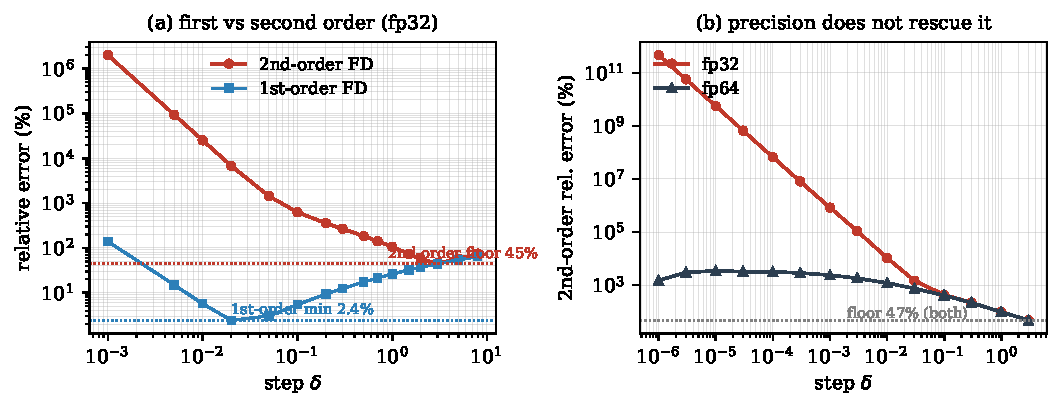
\includegraphics[width=\linewidth]{fig1_floor.pdf}
\caption{Non-recoverability of Proposition~\ref{prop:floor} on StyleGAN. The first-order
finite difference (blue) has a usable minimum; the second-order difference (red, mean over directions)
never falls below $\approx45\%$ at any common step, and the floor is identical in fp32 and fp64.}
\label{fig:floor}
\end{figure}

\section{An exact, step-free instrument}
\label{sec:inst}
The second-order term is the directional derivative of the first, so composing forward-mode AD with
itself,
\[
\partial^2_\alpha G(z+\alpha v)=\partial_\alpha\big[\partial G(z+\alpha v)[v]\big][v],
\]
is the exact derivative of the implemented graph and is evaluated by nesting two \jvp{} calls (in
PyTorch, \texttt{torch.func.jvp} of a function that returns a \jvp{}) \citep{paszke2019,griewank2008}.
At generator scale, the required object is the per-direction second-order pushforward of
the implemented network. Composed/forward-mode AD gives that object directly, building on
established ingredients -- Hessian-vector products at gradient cost \citep{pearlmutter1994},
hyper-dual numbers for exact second derivatives without a step \citep{fike2011}, and
second-order forward-mode AD \citep{baydin2018,cobb2024} -- and we use it here as the exact
reference against which finite differences are audited.
No Jacobian or Hessian is materialized, so memory is a small constant multiple of a single forward
evaluation -- about two for the second-order term -- rather than scaling with the output dimension, and
$k$ nested sweeps give the $k$-th-order pushforward. The instrument needs only a differentiable forward
graph and applies to any such architecture (a short per-generator adapter sufficed in our experiments). Its purpose here is to make the
prediction question of Section~\ref{sec:negative} answerable with the \emph{exact} second-order quantity,
so that whatever the answer turns out to be cannot be blamed on the estimator.

\section{A replication audit the instrument makes answerable}
\label{sec:negative}
We now use the exact instrument to ask a concrete question: does an edit direction's curvature
predict the estimator-free nonlinearity $\mathrm{NL}$ beyond the first-order displacement? This is
exactly the kind of audit the finite-difference estimator's step-selection ambiguity
(Section~\ref{sec:real}) would make uninterpretable, since a changed answer could be an artifact of
the estimator. The exact pushforward removes that ambiguity, so the answer is about the geometry. We use StyleGAN-bedroom,
$50$ edit directions (the $8$ annotated attribute boundaries plus $42$ random $w$-directions), and
average each quantity over $12$ latent anchors per direction; we repeat the entire correlation
across five independent anchor seeds and report the distribution. Rank correlations are Spearman;
partial correlations residualize ranks; confidence intervals are bootstrap over directions; the
first-order control of Section~\ref{sec:real} passes throughout ($2.4\%$).

\paragraph{A single anchor and a hand-picked subset cannot decide the question.} On one anchor
set restricted to $N{=}24$ \emph{named} directions -- a subset of the fifty, and a different
population from the full mixed set we use across anchors below -- exact curvature correlates with
nonlinearity at $\rho=0.47$ ($p=0.012$), with partial correlation $+0.45$ ($p=0.016$, $10^4$
permutations). This is not a robust signal: displacement and curvature are nearly collinear
($\rho_{c,J}=0.93$), two heavy-tailed directions carry it (removing them drops the raw correlation
to $0.31$, $p=0.075$), and it is computed on a hand-picked subset. We report it only as the
forking-paths trap it is -- a strong-looking number that the proper analysis below dissolves.

\paragraph{Across anchors the signal does not transfer.} On five anchors (50 directions
each, Figure~\ref{fig:neg}b) the partial correlation $\rho(\text{curv},\mathrm{NL}\mid\lVert
J_zv\rVert)$ is $+0.10,\,+0.19,\,-0.15,\,+0.37,\,+0.33$. We report both tests symmetrically. By
permutation the per-anchor $p$-values are $0.25,\,0.095,\,0.86,\,0.0038,\,0.010$, so the signal is
significant on two of five anchors, and both survivors clear a Bonferroni threshold of $.01$. By bootstrap, on the
other hand, every anchor's $95\%$ CI includes zero (e.g.\ seed $34$ $[-0.076,+0.648]$, seed $35$
$[-0.085,+0.611]$). The two tests do not agree -- permutation flags two anchors, every bootstrap CI
includes zero -- and with only $n=5$ anchors and CIs this wide the data are equally consistent with a
small positive effect and with none; the honest reading is that the signal does not transfer. The
cross-anchor mean partial is $+0.17$ (unweighted mean of
the five per-anchor estimates; $95\%$ CI from a Student-$t$ on $n=5$), $[-0.09,+0.43]$, falling to
$+0.06$ ($[-0.23,+0.34]$, median $+0.09$) once chord length is also controlled. So the effect does not transfer reliably to a new anchor.

\begin{figure}[t]\centering
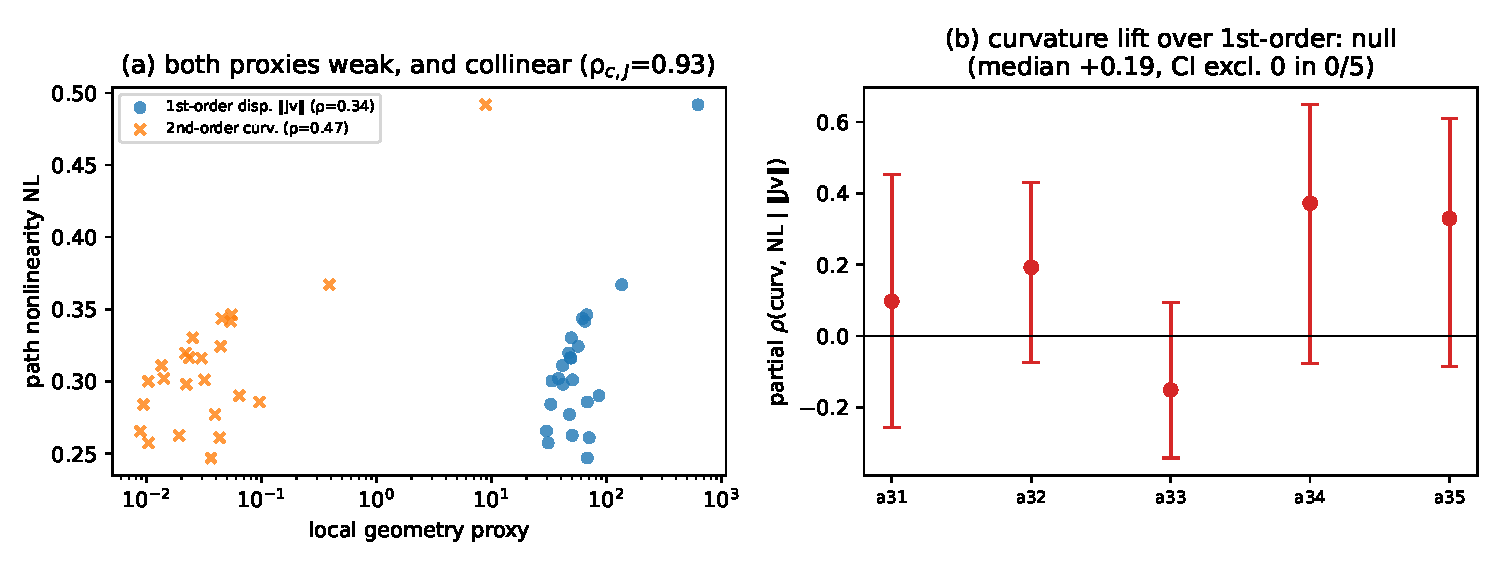
\includegraphics[width=\linewidth]{fig2_negative.pdf}
\caption{The exact second-order signal for edit nonlinearity is anchor-dependent and does not transfer.
(a) On a single anchor, first-order displacement and second-order curvature are nearly collinear
predictors of path nonlinearity. (b) Across five anchors, the partial correlation of curvature given
displacement is significant on $2/5$ by permutation (seeds $34,35$), while each
anchor's bootstrap $95\%$ CI includes zero; the cross-anchor estimate $+0.17$ has a CI that spans
zero, so the effect does not transfer.}
\label{fig:neg}
\end{figure}

\paragraph{Reading the audit.} The exact second-order signal is significant on two of
five anchors but does not transfer:
the second-order statistic should not be treated as anchor-stable without replication. The
$\geq45\%$ figure is a \emph{magnitude} error, whereas these audit correlations are rank/residual statistics. The
instrument-necessity is therefore the trilemma of Section~\ref{sec:real}: a fixed-step finite
difference's curvature
cannot be trusted for scale, sign, and ranking at once, and the practitioner cannot know in advance which
step preserves the property a given audit needs. A nuanced second-order effect is
therefore reliably auditable with an exact or step-validated reference, which removes the step choice.
We checked this confound directly: a fixed-step finite-difference curvature recovers the exact
direction ranking (Spearman $0.82$ at $\delta=3.0$ rising to $0.96$ at $\delta=0.1$) and two of the
three exact top directions at small steps (one of three at $\delta=3.0$), and against the
estimator-free nonlinearity it tracks the exact curvature ($\rho_{\mathrm{FD}}=0.19$--$0.35$ across
steps vs $\rho_{\mathrm{exact}}=0.47$) rather than flipping the verdict. So for this \emph{rank-level}
audit the two estimators agree on the (non-transferring) answer; the exact reference's necessity is on
the magnitude and sign axes (Section~\ref{sec:real}, Table~\ref{tab:trilemma}), where no step is
correct, not on this ranking question.

\paragraph{Why the question is a priori reasonable.} The result is not forced by collinearity:
the chord length -- raw global displacement -- is uncorrelated with nonlinearity ($\rho=0.065$), so
$\mathrm{NL}$ is not merely a re-encoding of how far the edit moves. The leading non-trivial term of
the chord deviation is $\tfrac12\alpha^2\partial^2_\alpha G$, so second-order curvature is the
\emph{a priori} right-order predictor of nonlinearity; the instrument lets us test that prediction
honestly rather than through the estimator's floor, and the honest answer is the mixed,
non-transferring one above.

\section{Recommendations, scope, and limitations}
\label{sec:scope}
\paragraph{Recommendation 1: use the exact instrument for second-order generator geometry.}
Probing second-order generator geometry calls for the exact instrument.
This is a deterministic consequence of Proposition~\ref{prop:floor}: a
finite-difference generator Hessian has a $\geq45\%$ relative-error floor on StyleGAN that no
step size or precision upgrade (including fp64) removes, while the composed-\jvp{} pushforward is exact to machine
precision at the cost of a small constant multiple of one forward pass. The same floor governs any
method built on a finite-difference second derivative of a generator. The Hessian Penalty
\citep{peebles2020} estimates exactly this second difference
$(1/\eps^2)[G(z+\eps v)-2G(z)+G(z-\eps v)]$; it is a stochastic training-time regularizer, so
averaging across samples may temper the error, but each per-sample estimate it averages sits on the
floor of Proposition~\ref{prop:floor}. For per-sample second-order measurement, the exact
composed-\jvp{} Hessian-vector product removes the step choice at a comparable constant number of
generator evaluations.

\paragraph{Recommendation 2: report the step axis when finite differences are used.}
If a finite-difference generator Hessian is used anyway, one tuned step is not enough evidence.
The report should show, or rule out, the three-way conflict we measure in Table~\ref{tab:trilemma}:
magnitude error, signed bias, and rank fidelity can be optimized at different steps. Without that
audit, the step choice can decide whether a magnitude, sign, or ranking conclusion holds.

\paragraph{Recommendation 3: replicate direction-level second-order claims across anchors.}
The replication audit in Section~\ref{sec:negative} shows the second failure mode: single-anchor
variability can decide whether a curvature correlation is significant. A second-order
generator-geometry claim should therefore pair an exact or validated estimator with replication
across anchors before treating a direction-level effect as stable.

\paragraph{On the audit.} The second-order signal for predicting edit nonlinearity is real in
aggregate but anchor-dependent (Section~\ref{sec:negative}); it does not transfer reliably across
anchors, so for a practitioner who cannot fix the anchor regime, first-order displacement
$\lVert J_z v\rVert$ -- a single \jvp{} -- is the safe default. That the signal is auditable at all
is itself a result for the instrument: a fixed-step finite difference cannot be trusted for the scale,
sign, and ranking of curvature at once (Section~\ref{sec:real}), so modest partial-correlation estimates
could not be reliably attributed to geometry rather than step choice without the exact reference.

\paragraph{Scope and limitations.} The prediction audit is confined to what we measured --
StyleGAN-bedroom, the path-nonlinearity target, and curvature versus first-order displacement -- and the
cross-anchor effect is modest ($+0.17$, CI spanning zero), so it stands only within this setting; we did
not run the nonlinearity-prediction study on FFHQ, diffusion U-Nets, or other targets such as identity
preservation and attribute leakage. The finite-difference trilemma is more broadly audited: it repeats on
two additional bedroom seeds, three full-resolution FFHQ seeds, and lower-detail FFHQ controls, but its
exact step values and floor heights are generator-dependent. The non-recoverability result
(Proposition~\ref{prop:floor}) is
architecture-independent and the instrument applies to any differentiable generator.

\section{Related work}
\label{sec:related}
Latent-geometry analyses of generative models use the first-order pullback metric $G=J^\top J$ to define
geodesics and argue that geodesic interpolation improves on linear interpolation
\citep{arvanitidis2018,shao2018,chen2018,yang2018}; these methods apply a curved path everywhere and rely
on the generator's higher-order structure without separating how reliably that structure can be computed.
Curvilinear editing \citep{aoshima2023} constructs nonlinear edit paths to be commutative. Second-order
information appears as a training-time disentanglement prior in the Hessian Penalty \citep{peebles2020},
which estimates the Hessian by exactly the finite-difference second difference our
Proposition~\ref{prop:floor} shows is non-recoverable. Closest to our object,
\citet{lee2023} regularize the explicit (extrinsic) curvature of a deep generative decoder
using second-order automatic differentiation, with a stochastic Hutchinson trace estimator
on low-dimensional autoencoders as a training-time prior; we instead compute the exact
per-direction second-order pushforward of pretrained production-scale generators as a
measurement instrument and quantify when the finite-difference alternative fails. Recent work computes curvature of generative
manifolds by careful grid finite differences \citep{koulakis2026}, a regime distinct from the
single-anchor second difference studied here. Our contribution is to identify the empirical
trilemma that this classical step-size analysis does not by itself settle on real generators:
finite differences cannot preserve curvature magnitude, sign, and rank with one defensible
step, while an exact composed-\jvp{} reference makes the resulting second-order claims auditable.
The numerical ingredients are established \citep{press2007,higham2002,pearlmutter1994,fike2011,griewank2008,baydin2018,cobb2024};
the new object is the generator-scale measurement decision they expose.

\section{Conclusion}
Finite differences cannot reliably recover the curvature of a generator. In single precision the central
second difference has a $\geq45\%$ magnitude-error floor that no step or precision removes
(Proposition~\ref{prop:floor}), and on a real generator this widens into an empirical step-selection
trilemma: the steps that best preserve magnitude, signed bias, and rank fidelity are different, while the
first-order quantity stays accurate, unbiased, and rank-faithful in a common step region
(Section~\ref{sec:real}). The exact composed-\jvp{} instrument recovers
it, to machine precision and at the cost of a small constant multiple of one forward pass. The
prescription follows directly: probing second-order generator geometry calls for the exact instrument,
since any method built on a finite-difference generator Hessian depends on an
unvalidated step choice. We then use the instrument to audit one practical question: a
single-anchor curvature--nonlinearity finding that looked strong becomes an aggregate but
non-transferring effect under anchor replication. That outcome is a decision rule for future
second-order reports: use an exact or step-validated estimator first, then replicate
direction-level claims across anchors before treating them as stable
\citep{locatello2019,hewitt2019}.

\section*{Reproducibility statement}
The submitted source archive contains the fixed-seed metrics behind every number in
Sections~\ref{sec:fd}--\ref{sec:negative}, the pure re-aggregation script for
Tables~\ref{tab:trilemma}--\ref{tab:fullsweep}, and the FFHQ runner scripts that record the
GPU protocols used for Table~\ref{tab:robustness}. The evidence directory contains the
per-anchor prediction tables, the per-record finite-difference sweeps, and the robustness
metrics and summaries. The Section~\ref{sec:negative} confound check (finite-difference versus
exact ranking and decision recovery) is reproduced by \texttt{30\_curvature\_ordering\_flip.py} and
\texttt{31\_curvature\_decision\_groundtruth.py} with their fixed-seed JSON outputs
(\texttt{curvature\_ordering\_flip\_metrics.json}, \texttt{curvature\_decision\_gt\_metrics.json}). The main generator is the public StyleGAN-bedroom-256 checkpoint
\citep{karras2019}; the robustness sweep uses the public InterFaceGAN StyleGAN-FFHQ semantic
boundaries and checkpoint at lod $0$--$2$ \citep{shen2020}. The generator runners require the
public checkpoints and repository wrappers; the fixed JSON artifacts allow the submitted
tables to be verified without rerunning GPU experiments. All experiments run on a single
8\,GB GPU.

\bibliography{refs}
\bibliographystyle{tmlr}

\newpage
\appendix
\section{Derivation of Proposition~\ref{prop:floor}}
\label{app:deriv}
Taylor expansion of $f(\alpha\pm\eps)$ to fourth order gives $D^2_\eps f = f''(\alpha) +
\tfrac{\eps^2}{12}f^{(4)}(\alpha)+O(\eps^4)$ for the exact arithmetic, the truncation term. In floating
point each evaluation carries error $O(\eps_{\mathrm{mach}}|f|)$; dividing the differenced numerator by
$\eps^2$ amplifies it to $O(\eps_{\mathrm{mach}}|f|/\eps^2)$, the cancellation term. Summing and
minimizing over $\eps$ gives $\eps^\star\sim(\eps_{\mathrm{mach}}C_R/C_T)^{1/4}\sim
\eps_{\mathrm{mach}}^{1/4}$ and floor $\sim\sqrt{C_TC_R\,\eps_{\mathrm{mach}}}$. The first difference
divides by $\eps$, giving cancellation $O(\eps_{\mathrm{mach}}|f|/\eps)$, optimum
$\eps_{\mathrm{mach}}^{1/3}$, floor $\eps_{\mathrm{mach}}^{2/3}$.

\section{Experimental setup}
\label{app:exp}
Path nonlinearity uses $T=3$ and $K=33$ render points. The second-order proxy is the mean absolute
$\partial^2_\alpha G$ via two nested \texttt{torch.func.jvp} calls; the first-order proxy is the \jvp{}
norm. The finite-difference trilemma sweep in Table~\ref{tab:trilemma} uses three HiGAN attribute
boundaries (indoor lighting, wood, view), three random unit $w$-directions, and $16$ base latents
(seed $31$) \citep{yang2020semantic}. Its robustness sweeps repeat the same bedroom protocol on seeds $32$ and $33$ and run an
analogous InterFaceGAN StyleGAN-FFHQ protocol \citep{shen2020} with five semantic boundaries, three random directions,
and $12$ base latents at full resolution (lod $0$, seeds $31$--$33$), plus lower-detail lod $1$ and $2$
controls (Appendix~\ref{app:robustness}). The multi-anchor
prediction analysis uses the $8$ HiGAN attribute boundaries (placed in their default manipulation layers)
and $42$ random unit $w$-directions, anchor seeds $31$--$35$, and $12$ base latents each; permutation tests
use $10^4$ resamples; bootstrap CIs use $2000$ resamples over directions.

\section{Full finite-difference step sweep}
\label{app:trilemma}
Table~\ref{tab:trilemma} in the body shows five representative steps. Table~\ref{tab:fullsweep} below
gives the complete $16$-step grid behind it, for both the second- and first-order finite differences
against the exact composed-\jvp{}, averaged over all $96$ direction--anchor pairs; the body's five rows
are a subset, not a selection. Each criterion's optimum (least magnitude error, least $|$signed bias$|$,
highest Spearman) is reached at a different second-order step, while the first-order columns are jointly
near-optimal across a broad region around $\delta=0.02$--$0.05$.

\begin{table}[h]\centering
\small
\begin{tabular}{r rrr rrr}
\toprule
& \multicolumn{3}{c}{second order (FD vs exact)} & \multicolumn{3}{c}{first order (FD vs exact)} \\
\cmidrule(lr){2-4}\cmidrule(lr){5-7}
step $\delta$ & mag.\ err & signed bias & Spearman & mag.\ err & signed bias & Spearman \\
\midrule
$8.0$   & $74.5\%$       & $-74.4\%$      & $0.712$ & $63.8\%$  & $-63.8\%$ & $0.687$ \\
$5.0$   & $57.3\%$       & $-55.6\%$      & $0.818$ & $54.0\%$  & $-54.0\%$ & $0.770$ \\
$3.0$   & $45.2\%$       & $-26.2\%$      & $0.897$ & $44.1\%$  & $-44.1\%$ & $0.867$ \\
$2.0$   & $56.1\%$       & $+4.9\%$       & $0.934$ & $37.1\%$  & $-37.1\%$ & $0.903$ \\
$1.5$   & $73.6\%$       & $+31.7\%$      & $0.950$ & $32.4\%$  & $-32.4\%$ & $0.924$ \\
$1.0$   & $106.4\%$      & $+76.1\%$      & $0.965$ & $26.2\%$  & $-26.2\%$ & $0.948$ \\
$0.7$   & $142.0\%$      & $+121.6\%$     & $0.975$ & $21.3\%$  & $-21.3\%$ & $0.967$ \\
$0.5$   & $184.2\%$      & $+170.3\%$     & $0.981$ & $17.4\%$  & $-17.4\%$ & $0.980$ \\
$0.3$   & $266.9\%$      & $+258.7\%$     & $0.983$ & $12.5\%$  & $-12.5\%$ & $0.991$ \\
$0.2$   & $355.2\%$      & $+350.4\%$     & $0.983$ & $9.4\%$   & $-9.4\%$  & $0.995$ \\
$0.1$   & $622.8\%$      & $+621.0\%$     & $0.970$ & $5.5\%$   & $-5.5\%$  & $0.999$ \\
$0.05$  & $1{,}429\%$    & $+1{,}429\%$   & $0.906$ & $3.1\%$   & $-2.9\%$  & $0.999$ \\
$0.02$  & $6{,}773\%$    & $+6{,}773\%$   & $0.721$ & $2.4\%$   & $-0.0\%$  & $0.999$ \\
$0.01$  & $25{,}023\%$   & $+25{,}023\%$  & $0.575$ & $5.7\%$   & $+4.5\%$  & $0.996$ \\
$0.005$ & $93{,}346\%$   & $+93{,}346\%$  & $0.527$ & $15.0\%$  & $+14.4\%$ & $0.986$ \\
$0.001$ & $1{,}985{,}856\%$ & $+1{,}985{,}856\%$ & $0.409$ & $139.1\%$ & $+139.0\%$ & $0.765$ \\
\bottomrule
\end{tabular}
\caption{Complete $16$-step finite-difference sweep on StyleGAN-bedroom ($96$ direction--anchor pairs),
second- and first-order, against the exact composed-\jvp{}. The second-order magnitude optimum
($\delta=3.0$), signed-bias optimum ($\delta=2.0$), and rank optimum ($\delta\approx0.2$--$0.3$) are at
distinct steps; the first-order quantity is jointly accurate, unbiased, and rank-faithful around
$\delta=0.02$--$0.05$.}
\label{tab:fullsweep}
\end{table}

\section{Robustness sweeps for the trilemma}
\label{app:robustness}
Table~\ref{tab:robustness} repeats the trilemma summary across two additional bedroom seeds, three
full-resolution StyleGAN-FFHQ seeds, and two lower-detail FFHQ controls. A separate FFHQ exact-\jvp{}
resolution audit preserves the ranking of semantic attributes across lod $0$, $1$, and $2$ (Spearman $1.0$
for each pair). The step values are generator-dependent. The repeated pattern is that the
second-order magnitude, signed-bias, and rank optima separate, while the first-order control
remains near a common small-step region.

\begin{table}[h]\centering
\small
\begin{tabular}{l r c c c c}
\toprule
sweep & $n$ & 2nd mag best & 2nd bias best & 2nd rank best & 1st stable \\
\midrule
bedroom seed 31 & $96$ & $3.0/45\%$ & $2.0/+5\%$  & $0.2/355\%$ & $0.02/2.4\%$ \\
bedroom seed 32 & $96$ & $3.0/51\%$ & $1.5/+11\%$ & $0.2/315\%$ & $0.02/2.2\%$ \\
bedroom seed 33 & $96$ & $3.0/43\%$ & $2.0/+5\%$  & $0.3/258\%$ & $0.02/2.3\%$ \\
FFHQ lod 0 seed 31 & $96$ & $5.0/71\%$ & $1.5/+2\%$  & $0.3/266\%$ & $0.02/8.0\%$ \\
FFHQ lod 0 seed 32 & $96$ & $5.0/71\%$ & $1.5/-8\%$  & $0.1/763\%$ & $0.02/7.2\%$ \\
FFHQ lod 0 seed 33 & $96$ & $5.0/69\%$ & $1.5/+1\%$  & $0.2/358\%$ & $0.02/7.5\%$ \\
FFHQ lod 1 seed 31 & $96$ & $8.0/74\%$ & $2.0/+12\%$ & $0.3/360\%$ & $0.02/10.0\%$ \\
FFHQ lod 2 seed 31 & $96$ & $8.0/72\%$ & $3.0/-13\%$ & $0.3/340\%$ & $0.02/8.7\%$ \\
\bottomrule
\end{tabular}
\caption{Robustness summary for the empirical step-selection trilemma. Each cell reports
step/error, except the bias column, which reports step/signed bias. The FFHQ rows test whether the
qualitative conflict survives a different generator and semantic-boundary set; the lod $1$ and $2$ rows
serve as lower-detail controls.}
\label{tab:robustness}
\end{table}

\end{document}
